% To produce pdf under linux, run
% pdflatex hw2.tex

% Credit for this template goes to Dr. Jerry Zhu.

\documentclass{article}
\usepackage[margin=1in]{geometry}
\usepackage{amsmath,amssymb}
\usepackage{bbm}
\usepackage{graphicx}
\usepackage{hyperref}
\usepackage{outlines}
\usepackage{enumitem}
\usepackage{float}
\usepackage{xcolor}
\usepackage{parskip}
\usepackage[skip=0.5\baselineskip]{caption}

\def\bfx{\mathbf x}
\def\R{\mathbb R}
\def\E{\mathbb E}
\def\argmax{\mathrm{argmax}}
\def\argmin{\mathrm{argmin}}


\newenvironment{soln}{
	\leavevmode\color{blue}\ignorespaces
}{}



\title{CS760 Spring 2019 Homework 2}
\author{Due Mar 7 at 11:59pm}
\date{}
\begin{document}
\maketitle


%%%%%%%%%%%%%%%%%%%%%%%%%%%%%%%%%%%%%%%%%%%%%%%%%%%%%%%%%%%%%%%%%%%%%%%%%
% Insert your name and email here:

Name: Stewart Kerr

Email: shkerr@wisc.edu 

%%%%%%%%%%%%%%%%%%%%%%%%%%%%%%%%%%%%%%%%%%%%%%%%%%%%%%%%%%%%%%%%%%%%%%%%%


\section*{Written Problems}

\textbf{NOTE:} For the following written problems, put your answer in \texttt{hw2.pdf}. You are required to provide detailed solutions including the intermediate results for each step. Otherwise, you will not get full credit. You can also add figures or tables whenever necessary. If your solutions are handwritten, make sure they are legible.

\begin{enumerate}
\item (8 pts) Suppose you have a Bayesian network with 6 binary random variables shown as follows, where \emph{t} and \emph{f} stand for \emph{true} and \emph{false} respectively.

Compute the probability: $P(d | b, \neg a, j, m)$.

\begin{figure}[h]
\centering
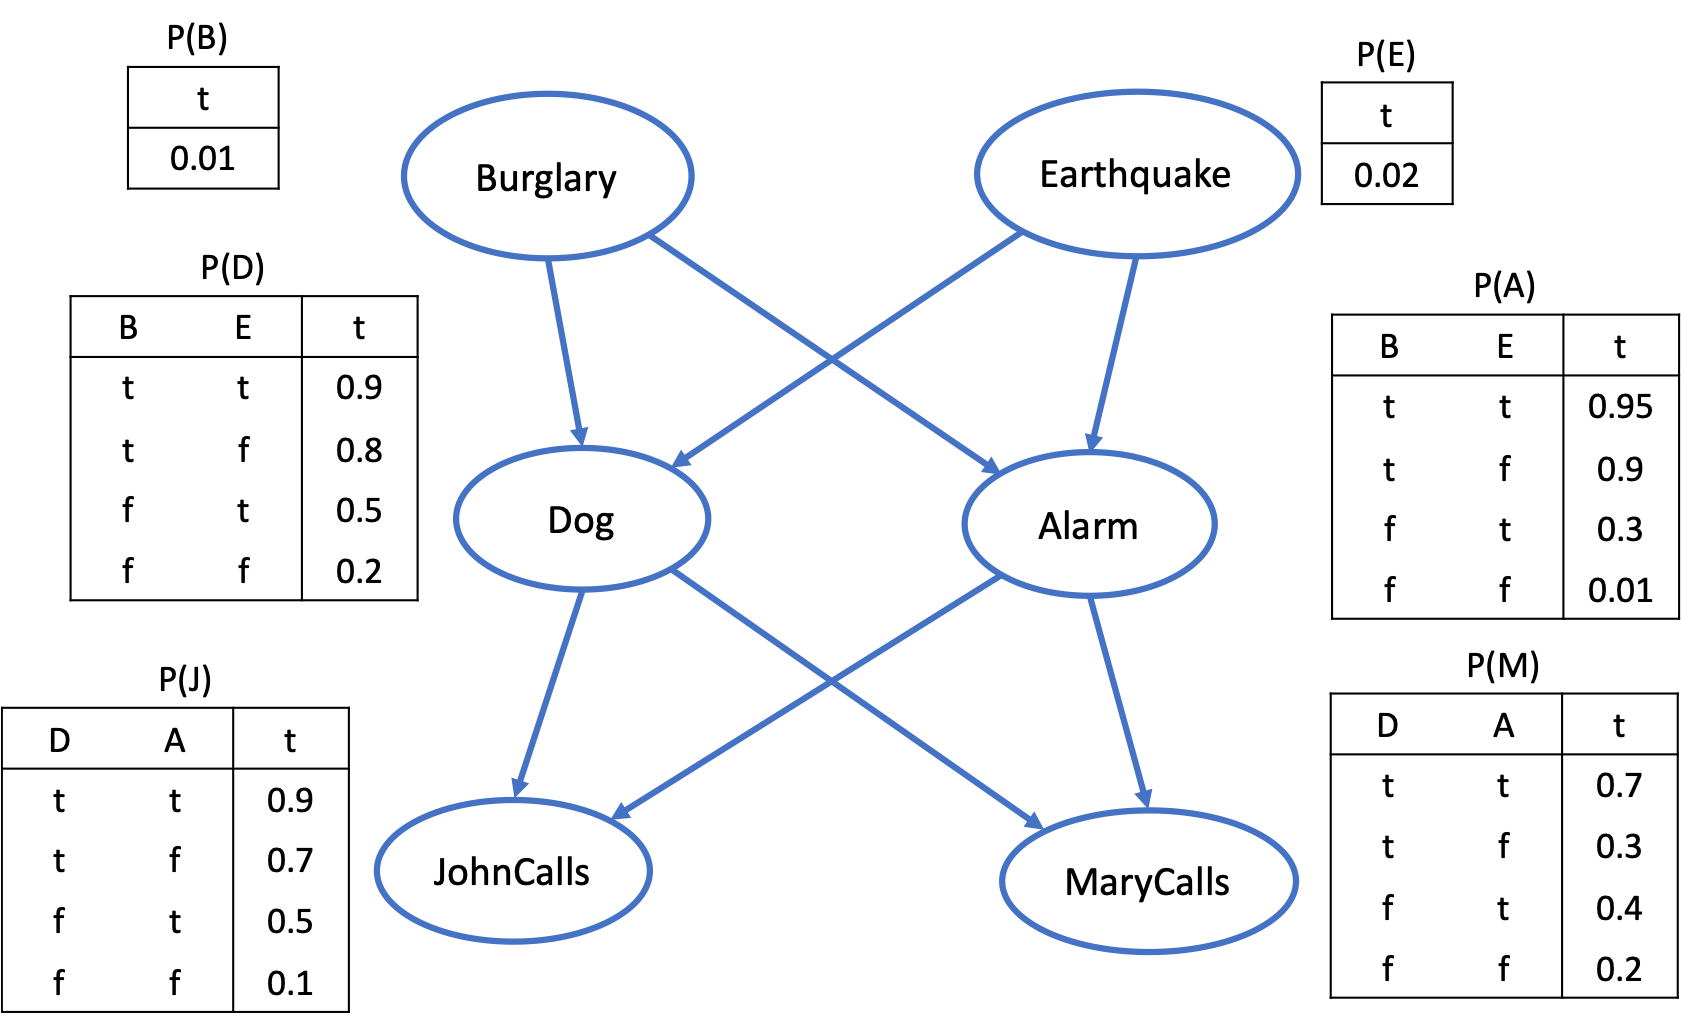
\includegraphics[scale=0.5]{figs/p1}
\label{fig:q1}
\end{figure}

\begin{soln}
From the formula of conditional probability, we know that $P(d | b, \neg a, j, m) = \frac{P(d, b, \neg a, j, m)}{P(b, \neg a, j, m)}$. \\ By the law of total probability, we can account for both earthquake outcomes and rewrite this fraction as  
\[ P(d | b, \neg a, j, m) = \frac{P(e,d, b, \neg a, j, m) + P(\neg e, d, b, \neg a, j, m)}{P(e, d, b, \neg a, j, m) + P(\neg e, d, b, \neg a, j, m) + P(e, \neg d, b, \neg a, j, m) + P(\neg e, \neg d, b, \neg a, j, m)} \]
Then, to get each probability in this sum, we just multiply the corresponding entries of the CPT (taking outcomes of dependent variables into account). Thus,
\[ P(e,d, b, \neg a, j, m) = P(e) \times P(b) \times P(d | e, b) \times P(\neg a | e, b) \times P(j | d, \neg a) \times P(m, d, \neg a) \]
\[ = 0.02 \times 0.01 \times 0.9 \times 0.05 \times 0.7 \times 0.3 = 1.89\times10^{-6}\] 
\[P(\neg e, d, b, \neg a, j, m) = 0.98 \times 0.01 \times 0.8 \times 0.1 \times 0.7 \times 0.3 = 0.00165\]
\[P(e, \neg d, b, \neg a, j, m) = 0.02 \times 0.01 \times 0.1 \times 0.05 \times 0.1 \times 0.2 = 2\times 10^{-8}\]
\[P(\neg e, \neg d, b, \neg a, j, m) = 0.98 \times 0.01 \times 0.2 \times 0.1 \times 0.1 \times 0.2 = 3.92\times 10^{-6}\]
Now, we plug all of those numbers into our equation for $P(d | b, \neg a, j, m)$.
\[P(d | b, \neg a, j, m) = \frac{1.89\times10^{-6} + 0.00165}{1.89\times10^{-6} + 0.00165 + 2\times 10^{-8} +  3.92\times 10^{-6}} = 0.977\]
Intuitively, this makes sense. If both John and Mary call, but the alarm did \textit{not} sound, then that places a higher "burden" on the dog barking to be the reason behind their calling. Thus, the probability that the dog barked will be higher.
\end{soln}

\pagebreak


\item Given the following Bayesian network and sample counts in each table, where sample counts \texttt{<n\textsubscript{true}, n\textsubscript{false}>}, there are \texttt{n\textsubscript{true}} samples with true labels and \texttt{n\textsubscript{false}} samples with false labels for this attribute. For example, \texttt{<138, 132>} in table \texttt{C|A} says given the condition of $A = true$, there are 138 instances are true and 132 are false with regard to attribute $C$.

You need to answer the following two questions.


\begin{figure}[H]
\centering
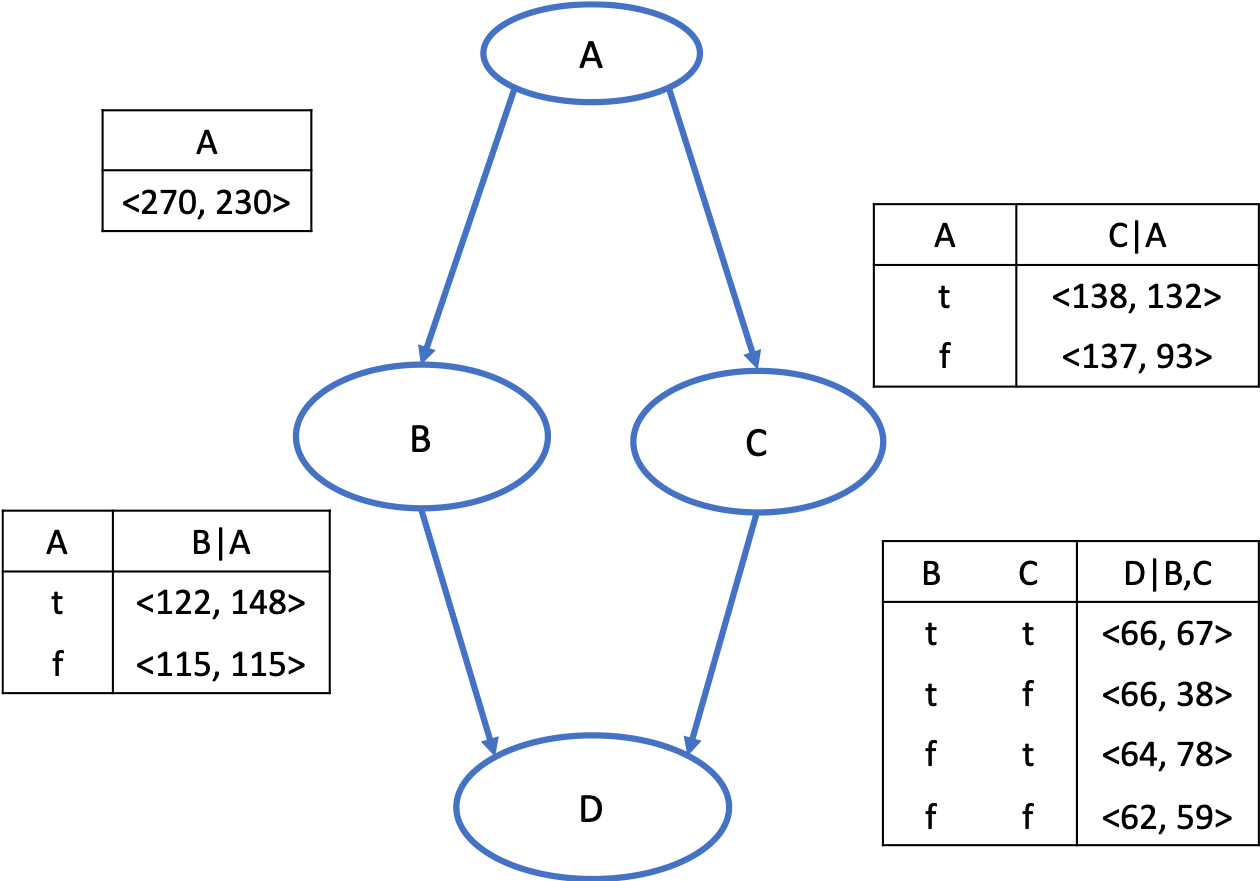
\includegraphics[scale=0.5]{figs/p2}
\label{fig:q2}
\end{figure}

\begin{enumerate}
\item (2 pts) Construct the conditional probability tables (CPTs) based on the above sample count tables, using maximum likelihood estimation. You need to both show the true probability \texttt{P\textsubscript{true}} and false probability P\textsubscript{false} for each case, and organize them in the format of \texttt{<P\textsubscript{true}, P\textsubscript{false}>}. For example, for the case \texttt{Y|X\textsubscript{1},X\textsubscript{2}}, your answer will look like \texttt{<P(Y|X\textsubscript{1},X\textsubscript{2}), P($\neg$Y|X\textsubscript{1},X\textsubscript{2})>}. Keep \textbf{at least 3 digits of precision.} (You may reuse the same structure as the above tables, just plugging in the conditional probabilities in the place of sample counts. For more information, please refer to the lecture notes \texttt{BNs-1.pdf})

\begin{soln}
See the figure below for the CPT tables.

\begin{figure}[h]
\centering
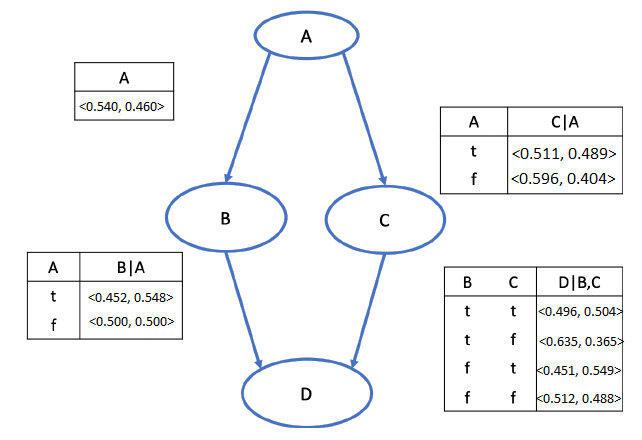
\includegraphics[scale=0.80]{figs/p2_ans}
\label{fig:q2_ans}
\end{figure}

\end{soln}



\vspace{10pt}

\item (10 pts) Show the result of one cycle of the EM algorithm to update the CPTs you derived in step (a), using 10 another instances with \texttt{A=true}, \texttt{B=false}, \texttt{C=?}, and \texttt{D=true} (`?' means missing value). Keep \textbf{at least 2 digits of precision}.

\begin{soln}
The EM algorithm has two steps - \\
E) Using the current CPT, calculate expected values of the missing data. \\
M) Update the model using the imputed values from E which maximize probability of the data

\textbf{Expectation step}
Given the CPT tables constructed above, we have 
\[P(c | a, \neg b, d) = \frac{P(a,\neg b, c, d)}{P(a,\neg b, c, d) + P(a,\neg b, \neg c, d)} = \frac{0.540\times0.548\times0.511\times0.451}{(0.540\times0.548\times0.511\times0.451) + (0.540\times0.548\times0.489\times0.512)}\]\[= 0.479\]
and
\[P(\neg c | a, \neg b, d) = 1 - P(c | a, \neg b, d) = 1 - 0.479 = 0.521\]
Thus, the expected counts for c and $\neg c$ using another 10 instances are $10\times0.479 = 4.79$ and $10\times 0.521 = 5.21$ respectively. \\

\textbf{Maximization step}
In the maximization step, we add the new data (with expected counts) to the previous counts and then recalculate the CPT table.
After adding the new data, the counts table is:
\begin{figure}[h]
\centering
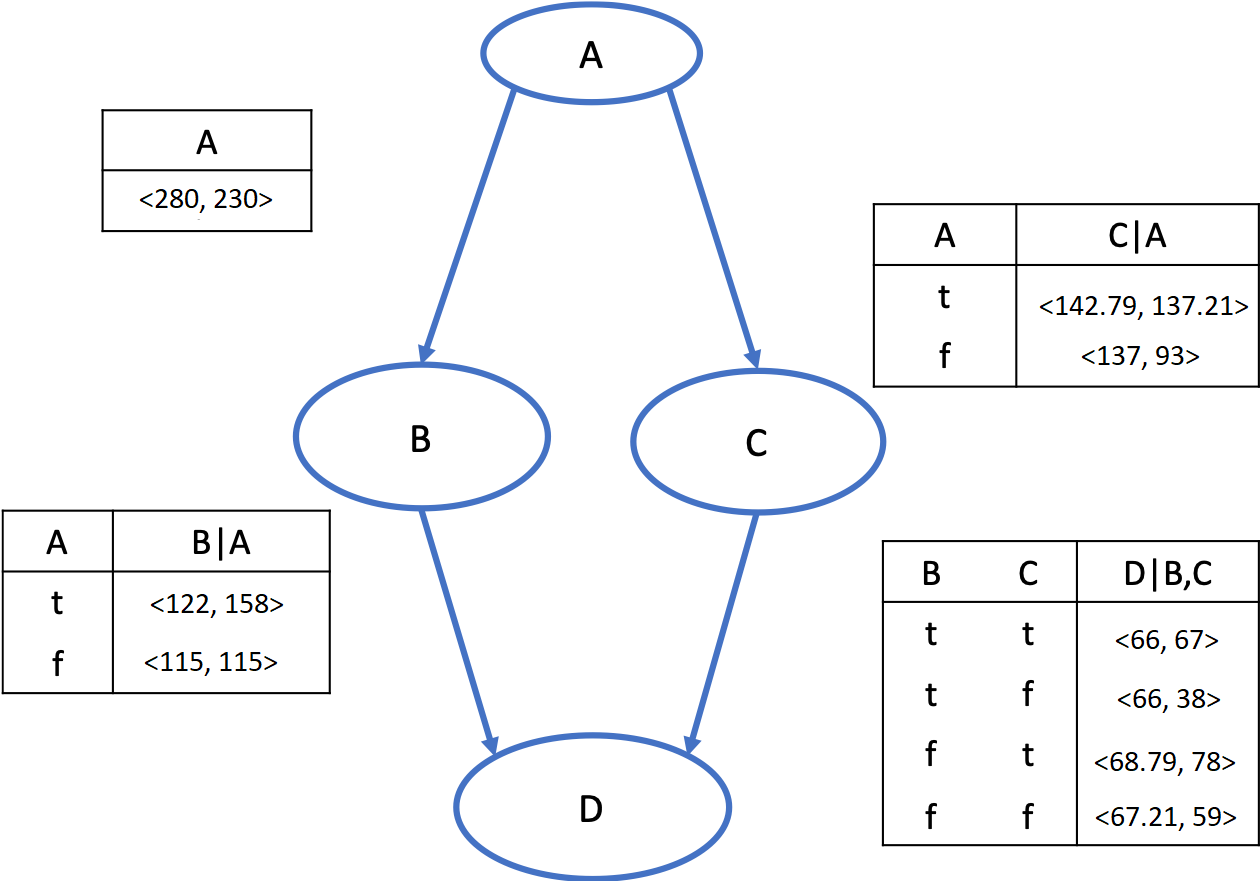
\includegraphics[scale=0.50]{figs/p2_ans2}
\label{fig:q2_ans2}
\end{figure}

\pagebreak
Thus, the new CPT table is:
\begin{figure}[h]
\centering
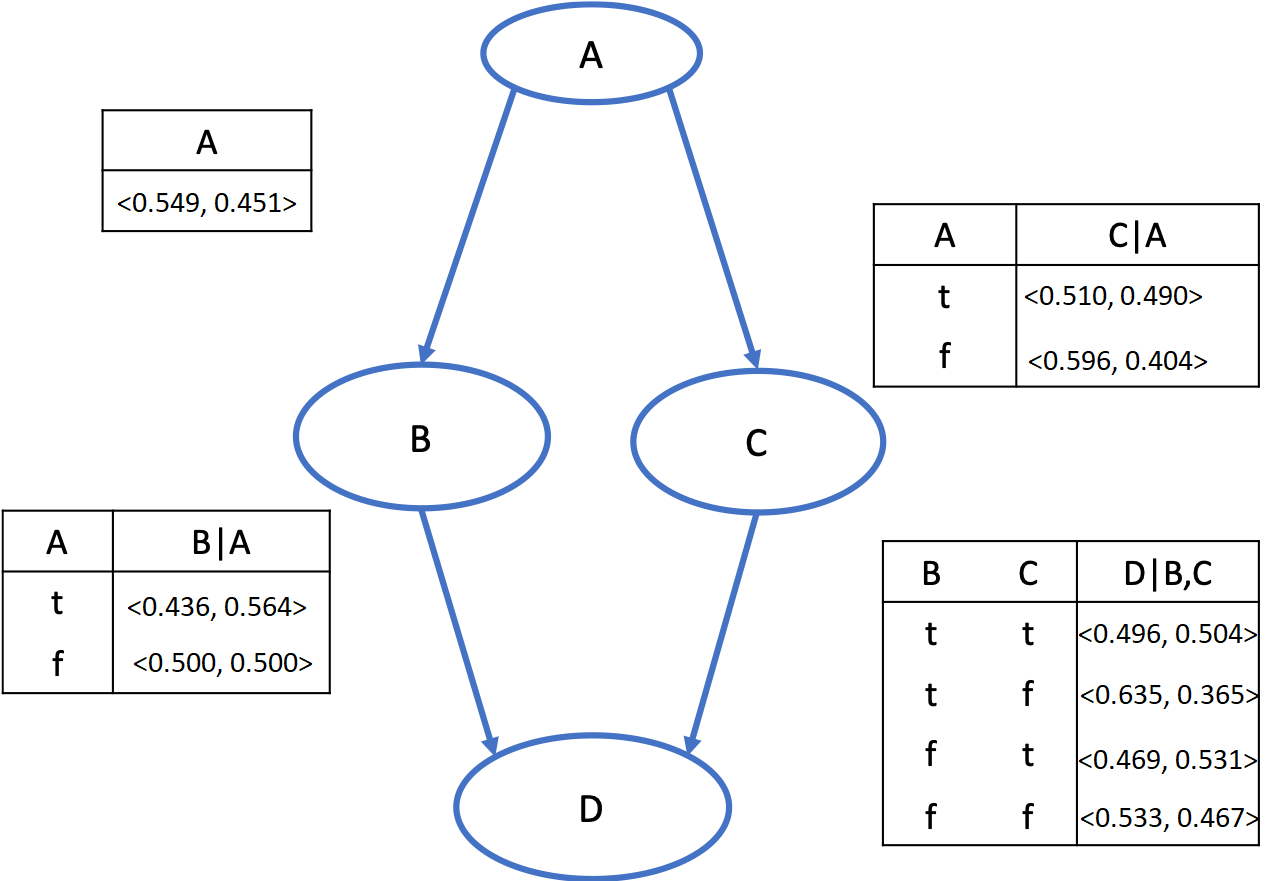
\includegraphics[scale=0.50]{figs/p2_ans3}
\label{fig:q2_ans3}
\end{figure}

\end{soln}



\end{enumerate}
\end{enumerate}


\end{document}
